\documentclass[12pt,a4paper,oneside,fleqn,leqno]{article}

\usepackage[utf8]{inputenc}
\usepackage[T2A]{fontenc}
\usepackage{amssymb,amsmath,mathrsfs,amsthm}
\usepackage[russian]{babel}
\usepackage{graphicx}
%\usepackage[footnotesize]{caption2}
\usepackage{indentfirst}
\usepackage{epstopdf}
\usepackage{multirow}
%\usepackage[ruled,section]{algorithm}
%\usepackage[noend]{algorithmic}
%\usepackage[all]{xy}
\usepackage[labelsep=period]{caption}
\usepackage[ruled,vlined,linesnumbered,algosection,algo2e]{algorithm2e}
\usepackage{paralist}
% Перевод плагина algorithm2e
\SetKwInput{KwData}{Исходные параметры}
\SetKwInput{KwResult}{Результат}
\SetKwInput{KwIn}{Входные данные}
\SetKwInput{KwOut}{Выходные данные}
\SetKwIF{If}{ElseIf}{Else}{если}{тогда}{иначе\ если}{иначе}{конец\ условия}
\SetKwFor{While}{до\ тех\ пор,\ пока}{выполнять}{конец\ цикла}
\SetKw{KwTo}{от}
\SetKw{KwRet}{возвратить}
\SetKw{Return}{возвратить}
\SetKwBlock{Begin}{начало\ блока}{конец\ блока}
\SetKwSwitch{Switch}{Case}{Other}{Проверить\ значение}{и\ выполнить}{вариант}{в\ противном\ случае}{конец\ варианта}{конец\ проверки\ значений}
\SetKwFor{For}{цикл}{выполнять}{конец\ цикла}
\SetKwFor{ForEach}{для\ каждого}{выполнять}{конец\ цикла}
\SetKwRepeat{Repeat}{повторять}{до\ тех\ пор,\ пока}
\SetAlgorithmName{Алгоритм}{алгоритм}{Список алгоритмов}

% Параметры страницы
\textheight=24cm
\textwidth=16cm
\oddsidemargin=5mm
\evensidemargin=-5mm
\marginparwidth=36pt
\topmargin=-1cm
\footnotesep=3ex
%\flushbottom
\raggedbottom
\tolerance 3000
% подавить эффект "висячих стpок"
\clubpenalty=10000
\widowpenalty=10000
\renewcommand{\baselinestretch}{1.5} %для печати с большим интервалом
\newcommand{\myparagraph}[1]{\paragraph{#1}\mbox{}\\}
\newcounter{pe} % новый счётчик
\newcommand*{\Nep}{\addtocounter{pe}{1}{\arabic{pe}$^{\circ}$.\;}}
\newcommand*{\NepS}{\mbox{} \\ \Nep}

% Список литературы - без [] -
\makeatletter\renewcommand{\@biblabel}[1]{#1.\hfill}\makeatother

\begin{document}

\begin{titlepage}
\begin{center}
    
\includegraphics[width=50mm]{msu.eps}

    \bigskip
	Московский государственный университет имени М.\,В. Ломоносова\\
	Факультет Вычислительной математики и кибернетики\\
	Кафедра Математических методов прогнозирования\\[20mm]

    {\large
        ДИПЛОМНАЯ РАБОТА\\[10mm]
\bfseries
        Управление динамическим объектом с использованием нейрокомпьютерного интерфейса
    }\\[10mm]

    \vfill

\begin{flushright}
  %\large
  \textbf{Автор:}\\
  студент 517 группы\\
  Зиннурова Эльвира Альбертовна

  \vspace{5mm}

  \textbf{Научный руководитель:}\\
  к.ф.-м.н., доцент\\
  Гуров Сергей Исаевич
\end{flushright}

\vfill

\begin{center}
Москва, 2015
\end{center}

\end{center}
\end{titlepage}

\newpage
\renewcommand{\contentsname}{Содержание}
\tableofcontents

\newpage
\begin{abstract}
	TODO: Написать аннотацию
    %Данный документ является образцом оформления дипломной работы для студентов кафедры 
    %Математических методов прогнозирования ВМК~МГУ. 
    %Приведённые ниже рекомендации взяты из~статьи
    %<<Написание отчётов и статей (рекомендации)>>
    %на~вики"~ресурсе \texttt{www.MachineLearning.ru}.
    %Студенты, готовящие дипломную работу к~защите, 
    %могут найти много полезной информации также в~статьях 
    %<<Научно-исследовательская работа (рекомендации)>>,
    %<<Подготовка презентаций (рекомендации)>>,
   % <<Защита выпускной квалификационной работы (рекомендации)>>
    %на~том~же ресурсе. 

    %Аннотация обычно содержит 
    %краткое описание постановки задачи и~полученных результатов,
    %одним абзацем на 10--15 строк.
    %Цель аннотации "--- обозначить в~общих чертах, о~чём работа,
    %чтобы человек, совершенно не~знакомый с~данной работой,
    %понял, интересна~ли ему эта тема, и~стоит~ли читать дальше.
    %Аннотация собирается в~последнюю очередь
    %путем легкой модификации наиболее важных и~удачных фраз из введения и~заключения.
\end{abstract}

\newpage
\section{Введение}
	\quad\,\,\,Нейрокомпьютерный интерфейс (англ. {\it brain-computer interface, mind-machine interface, brain–machine interface}, интерфейс «мозг-компьютер», зачастую используется сокращение {\it BCI}) ~--- специальный вид интерфейса, созданный для обмена информацией между мозгом и средствами вычислительной техники. Одной из задач, стоящих перед исследователями, работающими в данной области, является создание устройств, которые позволят людям с утраченными способностями организма полноценно взаимодействовать с окружающим миром.
	\par В последние годы ведётся активная разработка различных практических приложений с использованием интерфейса «мозг-компьютер». Многие исследовательские группы по всему миру занимаются тематикой {\it BCI}, и в разработке многих направлений тематики имеются заметные успехи, однако до сих пор существует масса сложностей в практическом применении нейрокомпьютерного интерфейса. Управление объектами реального мира может быть использовано в широком спектре областей, в частности, в медицине, развлекательной индустрии и пр.
	\par Тем не менее, на сегодняшний день распознавание воображаемых движений является стандартной задачей, разработаны алгоритмы, практически безошибочно классифицирующие ментальные задания, однако построенные системы {\it BCI} сложно назвать приспособленными для использования с практической точки зрения.
	\par Основной целью данной работы является построение модели нейрокомпьютерного интерфейса для управления динамическим объектом в некотором направлении с использованием общедоступного коммерческого устройства {\it Emotiv EPOC}. Кроме того, в данной дипломной работе проводится обзор существующих систем {\it BCI} и распространённых подходов к решению подобного рода задач.
	\par В первой главе даётся формальная постановка решаемой задачи.
	\par Далее описано используемое в данной работе оборудование, перечислены типы нейрофизиологических сигналов и объяснены причины, благодаря которым становится возможным решение поставленной задачи, а также обозначены имеющиеся на сегодняшний день проблемы при решении подобного рода задач.
	\par Затем перечислены и описаны алгоритмы, наиболее часто применяющиеся при решении задач в области нейрокомпьютерных интерфейсов, а также представлены наиболее распространённые методы сравнения систем {\it BCI}.
	\par После этого описывается процесс и методика получения данных в течение проводимых экспериментов, а также предлагаемый подход к распознаванию регистрируемых данных.
	\par Далее представлены полученные результаты и проведено сравнение полученной точности с аналогичными исследованиями в данной области, а также приведены основные выводы, сделанные по результатам имевших место исследований.

\clearpage 

\section{Постановка задачи}
	\quad\,\,\,Целью данной работы является построение модели нейрокомпьютерного интерфейса для управления динамическим объектом в некотором направлении с использованием общедоступного коммерческого устройства {\it Emotiv EPOC}, предназначенного для регистрации активности головного мозга при помощи зафиксированных сенсоров. Данное устройство подробно описано в разделе~\ref{Emotiv_descr}.
 	\par Пусть имеется $M$ сенсоров, в моменты времени $1, 2, \dots, t, \dots$ $i$-ый сенсор фиксирует значения $x^i(t)$, $i = \overline{1,M}.$ Требуется определить класс регистрируемого в произвольный момент времени $t$ сигнала, в частности, в данной работе в качестве классов выступают возможные направления движения курсора. Обычно полагают, что многомерный сигнал разбит на отрезки фиксированной длины $T$, на протяжении каждого из которых класс сигнала остаётся неизменным. Везде далее будем придерживаться данного предположения.
	\par Дадим формальную математическую постановку задачи.
	\par Имеется пространство объектов $\mathcal{X} \subset \mathbb{R}^{M \times T}$, каждый из которых представляет собой сигнал, зафиксированный при помощи $M$ сенсоров в течение периода времени $T$, и конечное множество имён классов $\mathcal{Y}$. Существует целевая зависимость $y^*: \mathcal{X} \to \mathcal{Y},$ значения которой известны только на объектах обучающей выборки $X^L = \{ (x^i, y^i)\}_{i=1}^L, \, x^i \in \mathcal{X} \subset \mathbb{R}^{M \times T}, \, y^i = y^*(x^i) \in \mathcal{Y}, \, L$ -- количество объектов обучающей выборки. Требуется построить алгоритм классификации $a: \mathcal{X} \to \mathcal{Y},$ аппроксимирующий целевую зависимость $y^*(x)$ на всем множестве $\mathcal{X}$ в соответствии с некоторым введённым функционалом качества.

\clearpage 

\section{Нейрокомпьютерные интерфейсы}
	\subsection{Используемое оборудование}\label{Emotiv_descr}
	\par Главная цель исследований в области нейрокомпьютерных интерфейсов -- разработка систем, позволяющих обездвиженным пользователям обмениваться информацией и взаимодействовать с другими людьми, а также контролировать различные элементы их окружения. Кроме того, подобные системы могут быть использованы для улучшения контроля над сложными многозадачными операциями.
	\par Нейрокомпьютерный интерфейс -- средство коммуникации, транслирующее активность головного мозга в действия либо команды, исполняемые электронными устройствами. Фиксация подобного рода активности становится возможной вследствие физико-химических процессов, лежащих в основе обмена веществ в нервной ткани, порождающих колебания потенциалов головного мозга. Несмотря на то что существует множество различных методов фиксации активности головного мозга (электрокортикография\footnote{{\it Электрокортикография} — метод отведения потенциалов при помощи электродов, накладывающихся непосредственно на кору головного мозга. Потенциалы имеют на порядок большую амплитуду по сравнению с ЭЭГ, а также лучшее разрешение.}, электроокулография\footnote{{\it Электроокулография} — исследование глазных мышц и наружного слоя сетчатки благодаря изменениям биопотенциалов во время движения глаза и стимуляции сетчатки, и переводу зарегистрированных изменений в графическое представление.} и др.), в настоящее время основным способом получения сигналов головного мозга является электроэнцефалография. 
	\par {\it Электроэнцефалография (ЭЭГ)} — раздел электрофизиологии, изучающий закономерности суммарной электрической активности мозга, отводимой с поверхности кожи головы или мозга, а также метод записи таких потенциалов. Получение электроэнцефалограммы осуществляется с помощью специализированных устройств -- электроэнцефалографов. Существуют различные устройства для записи ЭЭГ, отличающиеся характеристиками, среди которых: 
	\begin{itemize}\itemsep0pt
	\item
	характеристики принимающего сигнала (частота, количество шума в сигнале);
	\item
	инвазивность (степень имплантирования электродов в кору головного мозга);
	\item
	количество электродов;
	\item
	покрываемая площадь (среднее количество влияющих на сигнал нейронов, снимаемый одним электродом).
	\end{itemize}
	\par По инвазивности устройства делятся на {\it погружные}, {\it частично-погружные} и {\it непогружные} в зависимости от расположения электродов (электроды вживлены в мозг/сращены с нервами, находятся на поверхности мозга/рядом с нервами или находятся на поверхности кожи головы соответственно).

	\par Устройства с непогружным интерфейсом делятся на {\it мокрые} и {\it сухие} в зависимости от того, необходимо ли смачивание электродов проводящей жидкостью для осуществления контакта.
	\par По типу электродов устройства делятся на {\it пассивные} и {\it активные} в зависимости от того, производится ли после снятия электродом сигнала его первичная обработка.

	
	\par В настоящей работе для записи электроэнцефалограммы использовалось устройство {\it Emotiv EPOC}. Это устройство было разработано австралийской компанией {\it Emotiv Systems}, основанной в 2003 году. Данная компания входит в число трёх основных участников рынка потребительских устройств {\it BCI} наряду с компаниями {\it NeuroSky} и {\it OCZ}, однако {\it Emotiv EPOC} имеет значительно большее число электродов, чем устройства компаний-конкурентов, и незначительно более высокую стоимость. 
\begin{figure}[h!]
\center{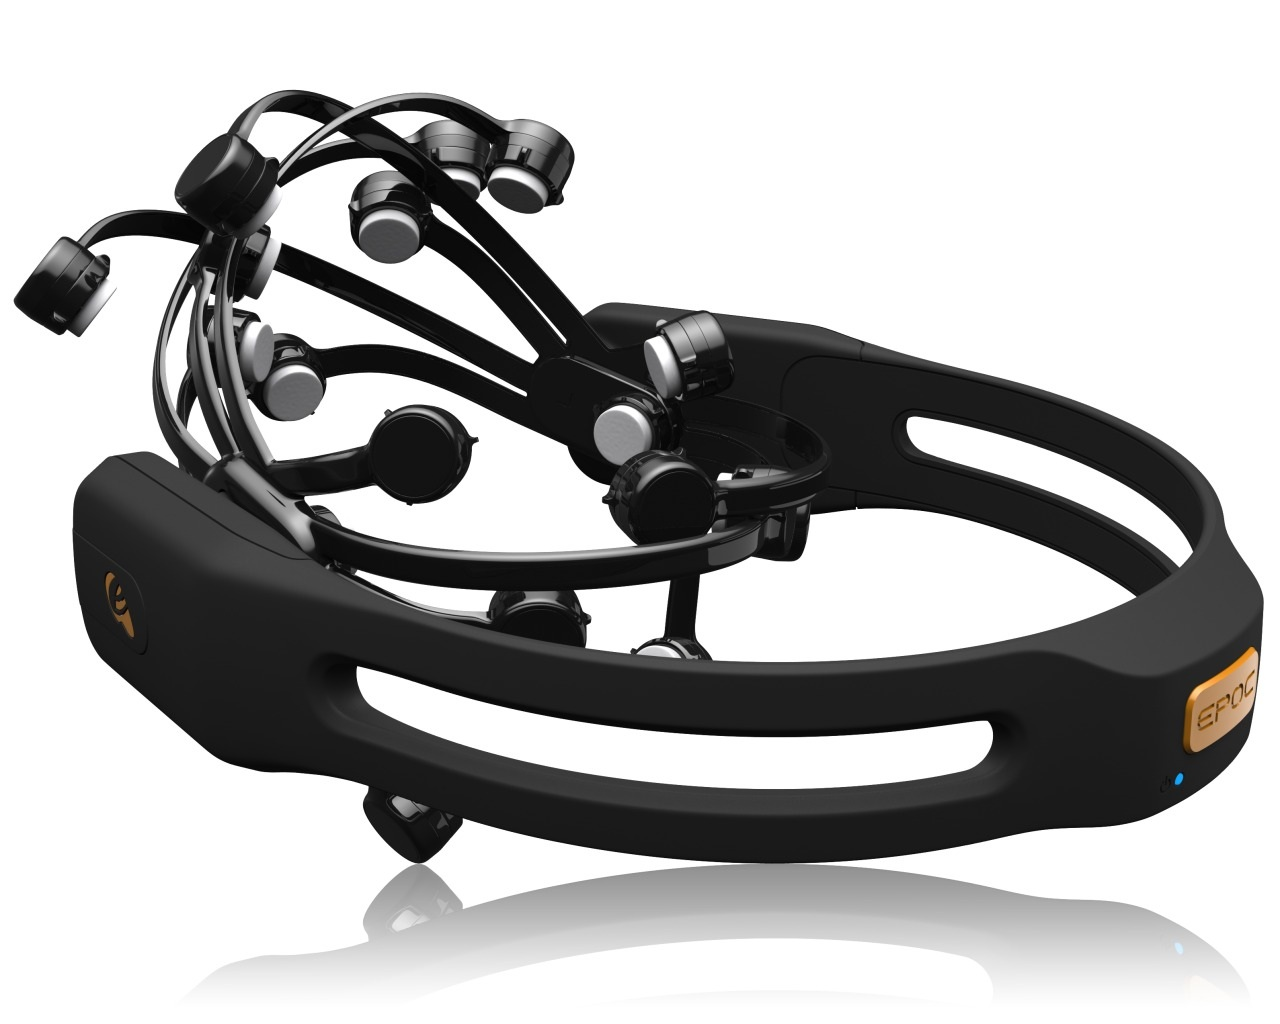
\includegraphics[width=1\linewidth]{Emotiv.jpg}}
\caption{{\it Emotiv EPOC} ~--- устройство, используемое для записи данных ЭЭГ.}
\label{Emotiv}
\end{figure}

	\par Общий вид устройства изображён на рис.~\ref{Emotiv}, устройство обладает следующими характеристиками:
	\begin{itemize}\itemsep0pt
	\item
	число датчиков — 14;
	\item
	тип датчиков — пассивные, мокрые;
	\item
	частота дискретизации — 128 Гц;
	\item
	способ связи — беспроводная радиосвязь;
	\item
	гироскопы — 2 шт.;
	\item
	инвазивность — непогружной.
	\end{itemize}

	\par Расположение сенсоров устройства в соответствии с системой размещения электродов <<10 -- 20\%>>\footnote{Система «10—20\%» — стандартная система размещения электродов на поверхности головы, рекомендованная Международной федерацией электроэнцефалографии и клинической нейрофизиологии. Подробное описание данной системы может быть найдено в~\cite{system10-20}.} изображено на рис.~\ref{electrode_map}.

	\par Устройство {\it Emotiv EPOC} было использовано в силу своей простоты и доступности. Также достоинствами данного устройства являются портативность и небольшие размеры. В то же время оно обладает и рядом недостатков: низкая точность снимаемого сигнала и ненадёжная фиксация устройства на голове человека. В рамках настоящей работы будет предпринята попытка купировать недостатки устройства применяемыми методами обработки и классификации сигнала.

	\begin{figure}[h!]
	\center{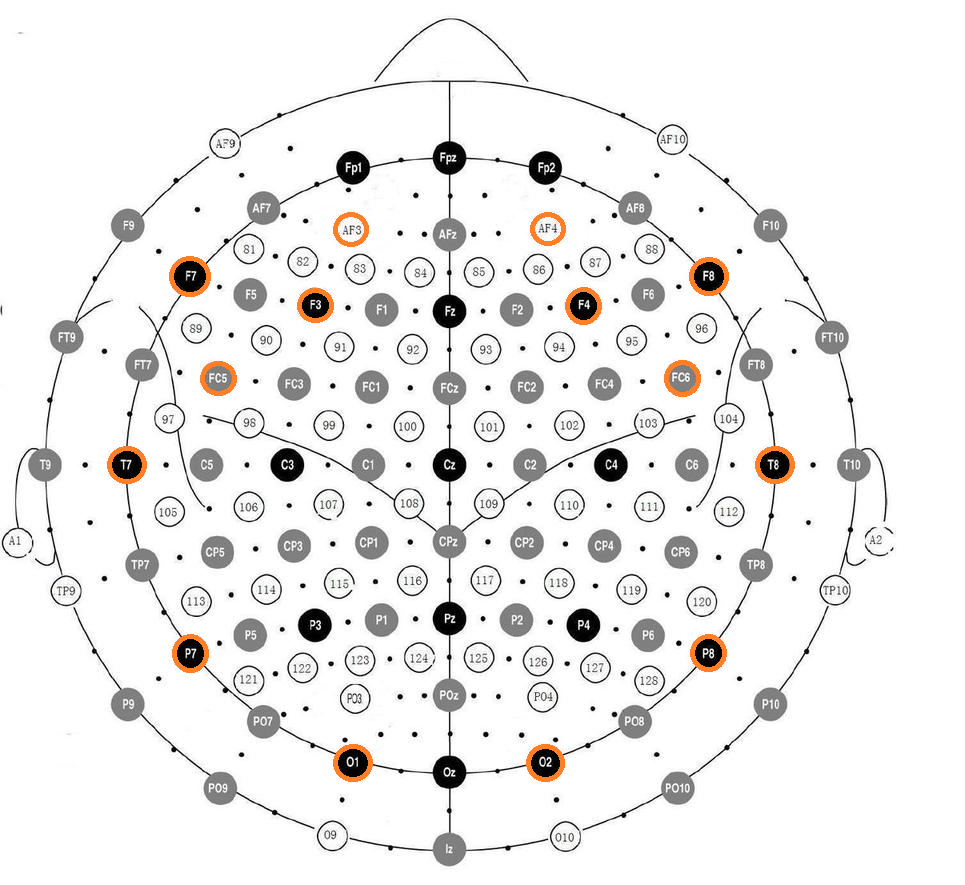
\includegraphics[width=0.9\textwidth]{electrode_map_1020.png}}
		\caption{Расположение электродов на голове человека согласно международной системе размещения электродов <<10--20>>. Электроды устройства {\it Emotiv EPOC} выделены оранжевым цветом.}
	\label{electrode_map}
	\end{figure}

	\subsection{Типы нейрофизиологических сигналов}
	\par Предполагается, что идеализированный нейрокомпьютерный интерфейс будет напрямую транслировать всякое намерение пользователя и посылать сигнал управляемому устройству о выполнении соответствующего действия. Однако установление однозначного соответствия между намерениями пользователя и нейрофизиологическими сигналами является нетривиальной задачей. На сегодняшний день данный факт является одной из основных причин ограничения свободы действий в существующих системах {\it BCI}.
	\par Для распознавания различных нейрофизиологических сигналов и возможности сопоставления подобного рода сигналов и подразумеваемых действий необходимо осознанное управление активностью головного мозга. В основном для достижения этой цели используются два подхода. При использовании первого подхода испытыемые подвергаются воздействию набора стимулов нейрокомпьютерного интерфейса, и контроль мозговой активности осуществляется путём концентрации на одном конкретном стимуле. Изменения нейрофизиологических сигналов в силу различий между стимулами называются {\it вызванными потенциалами} (англ. {\it event-related potentials, ERPs}). При использовании второго подхода управление мозговой активностью осуществляется путём выполнения определённого когнитивного (ментального) задания, например, представления определённого движения руки может явиться причиной изменения активности в соответствующей части скальпа.\\
	\setcounter{pe}{0}
	\NepS {\bf Вызванные потенциалы}
	\par Вызванный потенциал — электрическая реакция мозга на внешний раздражитель или на выполнение некоторого ментального задания. Потенциалы данного вида имеют место в течение определённого промежутка времени после воздействия стимула.
	\paragraph{Волны P300.}
	\parВолна P300 -- положительное отклонение сигнала ЭЭГ, имеющее место приблизительно через 300 мс после воздействия стимула с малой вероятностью появления, описывающего некоторое действие. Для порождения подобного рода волн испытуемому требуется пронаблюдать последовательность двух типов стимулов. Первый тип стимулов (т.н. {\it целевые} стимулы) являются редкими в последовательности стимулов, в отличие от другого типа стимулов (т.н. {\it нецелевые} стимулы). Таким образом, во время появления целевого стимула может быть зафиксирована мозговая активность, содержащая волны P300. Данный принцип был применен в системе {\it BCI}, разработанной в исследовании \cite{Farwell_Donchin}. В данном исследовании было описано устройство для набора текста. На экране изображалась таблица доступных для набора символов, строки и столбцы которой выделялись в случайном порядке, в качестве целевого стимула выступало выделение столбца/строки с желаемым на данный момент символом, в качестве нецелевых стимулов -- выделение остальных столбцов/строк.
	\paragraph{Визуальные вызванные потенциалы.}
	\par Визуальные вызванные потенциалы (англ. {\it Steady-State Visual Evoked Potentials}, {\it SSVEPs}) -- осцилляции, имеющие место в данных, полученных при помощи сенсоров, расположенных на затылке. Данные изменения могут быть результатом однородного процесса, повторяющегося с малой частотой. Подобного рода стимуляция порождает колебания той же частоты в регистрируемых сигналах головного мозга. В исследованиях по тематике нейрокомпьютерных интерфейсов потенциалы этого типа используются при одновременной демонстрации стимулов с разной частотой. Таким образом, пользователь путём концентрации на конкретном стимуле имеет возможность выбора действия, соответствующего данному стимулу.\\
	\paragraph{Моторные вызванные потенциалы.}
	\par Моторные вызванные потенциалы (англ. {\it Motor-Related Potentials}, {\it MRPs}) -- продолжительные отрицательные потенциалы, связанные с ожиданием или ментальным представлением выполняемого движения или действия, имеют место в сенсомоторной части скальпа в начале выполнения движения или в процессе ментального представления движения.
	\\ \NepS {\bf Частотная мозговая активность}
	\par В электроэнцефалограмме здорового человека выделяют несколько характерных составляющих электрических колебаний, называемых {\it ритмами}, различающихся частотным диапазоном, а также амплитудой, формой волны и другими характеристиками. Считается, что каждый ритм соответствует некоторому определённому состоянию мозга и связан с определёнными церебральными механизмами, а потому выделение ритмов, представляющих интерес, исходя из априорных знаний, может быть использовано для декодирования намерений пользователя.

\begin{table}[h]
\centering
\begin{tabular}{|c|c|}
\hline
Ритм & Частота (Гц) \\ \hline
$\delta$-ритм & 1-4 \\ \hline
$\theta$-ритм & 4-7 \\ \hline
$\alpha$-ритм & 7-13 \\ \hline
$\beta$-ритм & 13-30 \\ \hline
$\gamma$-ритм &  30+ \\ \hline
\end{tabular}
\caption{Частотные полосы наиболее изученных ритмов ЭЭГ.}
\end{table}

	\paragraph{Сенсомоторные ритмы.}
	\par Колебания $\mu$-ритма могут быть обнаружены в сенсомоторной части скальпа, когда пользователь находится в состоянии покоя. Если же выполняется некоторое фиксированное движение или ментальное представление данного движения, амплитуда колебаний уменьшается. Кроме того, подобные действия также порождают изменения в амплитуде $\beta$-ритма. Изменения данных ритмов отражаются на части скальпа, отвечающей перемещаемой части тела, в связи с этим представляемые и выполняемые движения различных частей тела могут быть отличимы друг от друга.
	\par Имеющие место изменения мозговой активности для пользователей с небольшим опытом использования нейрокомпьютерных интерфейсов обычно оказываются недостаточно весомыми для адекватного функционирования распознающих алгоритмов. Кроме того, используемое в данном исследовании устройство не покрывает часть скальпа, отвечающую за генерацию волн, связанных с подобного рода событиями. В связи с этим в дальнейшем данный подход не будет рассматриваться.

	\paragraph{Прочая активность.}
	\par В качестве триггеров возникновения колебаний потенциалов могут быть использованы когнитивные задания, отличные от представления движений, например, вычисления, слуховые представления, представление движения трёхмерного объекта в пространстве и др.

	\subsection{Нейрокомпьютерные интерфейсы на основе волн P300}
	\setcounter{pe}{0}
	\NepS {\bf Вызванные потенциалы и волны P300}
	\par Волны P300 были открыты в исследовании \cite{P300_first} в 1965 году. С тех пор имело место множество исследований по изучению природы этих колебаний путём изменения различных характеристик проводимых экспериментов, таких как способ демонстрации стимула, пол, возраст испытуемых, наличие заболеваний  и пр.
	\par Существуют исследования, описывающие подходы к управлению динамическим объектом при помощи моторных и визуальных вызванных потенциалов, однако в рамках данной работы в качестве объектов для принятия решения будут выступать волны P300, поскольку используемое оборудование не покрывает участок скальпа, отвечающий за моторные вызванные потенциалы, а визуальные вызванные потенциалы были сочтены не соответствующими поставленной задаче с практической точки зрения.
	\par Различные парадигмы могут быть использованы для выявления волн P300. В качестве стимулов могут быть использованы слуховые, визуальные, тактильные, обонятельные, вкусовые стимулы. Тем не менее, чаще всего используются визуальные и слуховые стимулы, а также их сочетания, поскольку данные типы являются лучшим выбором с практической точки зрения. В основном в большинстве исследований применяются две парадигмы проведения экспериментов: оригинальная (англ. {\it oddball paradigm}) и трёхстимульная (англ. {\it three-stimulus paradigm}).
	\par Оригинальная парадигма подразумевает использование двух типов стимулов (целевых и нецелевых), демонстрируемых в произвольном порядке, причём демонстрация целевого стимула является гораздо более редким событием по сравнению с демонстрацией нецелевого стимула. Испытуемымому же необходимо концентрироваться исключительно на целевом стимуле и игнорировать появление нецелевых стимулов.
	\par Трёхстимульная парадигма является модификацией оригинальной парадигмы. В~данном случае помимо описанных типов стимулов также присутствуют т.н. {\it отвлекающие} стимулы, редко появляющиеся в последовательности целевых и нецелевых стимулов. Испытуемые не информируются о наличии подобного рода стимулов в процессе инструктажа.
	\par При использовании описанных парадигм наблюдаются различные типы волн P300. Применение оригинальной парадигмы позволяет обнаружить т.н. волны P3b, имеющие место приблизительно в течение 300-500 мс после воздействия целевого стимула при концентрации на таковом. При использовании же трёхстимульной парадигмы целевой стимул также порождает волны P3b, при этом отвлекающий же стимул порождает другой тип волны P300, называемый волной P3a, имеющей место приблизительно в течение 200--400 мс после воздействия стимула. Характер возникновения волн каждого из описанных типов в процессе проведения эксперимента с использованием различных парадигм изображен на рис.~\ref{paradigms}.
\newline

\begin{figure}[h!]
\begin{minipage}[h!]{0.47\linewidth}
\center{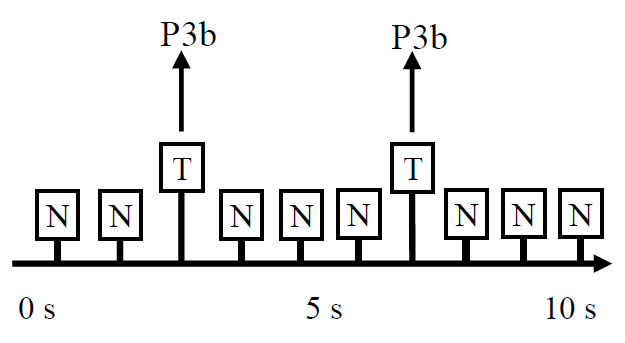
\includegraphics[width=1\linewidth]{oddball.png} \\ а)}
\end{minipage}
\hfill
\begin{minipage}[h!]{0.52\linewidth}
\center{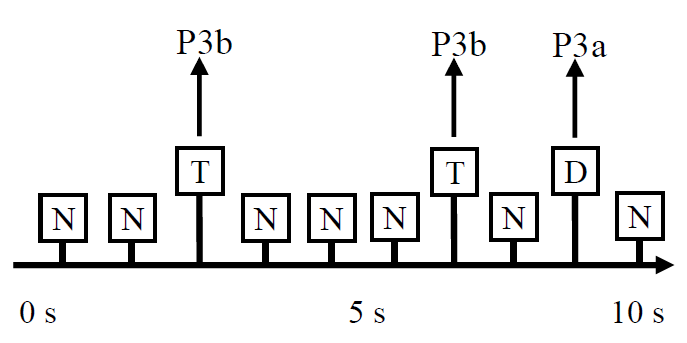
\includegraphics[width=1\linewidth]{3stim.png} \\ б)}
\end{minipage}
\caption{Оригинальная (а) и трёхстимульная (б) парадигмы проведения экспериментов с порождением волн P300.}
\label{paradigms}
\end{figure}

	\NepS {\bf Влияние различных факторов на волны P300}
	\par Кроме влияния различных экспериментальных парадигм, упомянутых выше, волны P300 также подвержены влиянию многих других факторов~\cite{P300_eval}~\cite{P300_effects}~\cite{P3a_effects}, перечисленных ниже.
	\paragraph{Веростность появления целевого стимула.} Амплитуда волны P3b обратно пропорциональна вероятности появления целевого стимула: редкое появление целевого стимула порождает высокий пик волны, в то время как высокая вероятность появления стимула слабо отражается на сигнале. В основном при проведении экспериментов вероятность появления данного типа стимулов полагается примерно равной 10\% для более надёжного выявления волн P300.  Кроме того, на амплитуду волны P3b также влияет локальная вероятность появления целевого стимула.
	\paragraph{Межстимульный интервал.} Амплитуда волны P3b прямо пропорциональна продолжительности межстимульного интервала (периода времени между двумя последовательными воздействиями стимулов).
	\paragraph{Привыкание.} Амплитуда волны P3a снижается с течением времени, поскольку из-за воздействия большого количества отвлекающих стимулов данное событие становится ожидаемым для испытуемого. В то же время амплитуда волны P3b практически не подвержена влиянию этого фактора.
	\paragraph{Степень концентрации.} Амплитуда волны P3b в большой мере зависит от степени концентрации пользователя. Более детально, волны P3b полностью исчезают, если пользователь не вовлечен в активное выполнение заданий. В то же время волны P3a не подвержены влиянию данного фактора.
	\paragraph{Сложность заданий.} Латентность волны P3b прямо пропорциональна сложности выполняемого  задания, в то время как амплитуда обратно пропорционально этой величине. К примеру, целевые стимулы, сильно отличающиеся от нецелевых, ведут к более высокой амплитуде волны P3b по сравнению со случаем слабых отличий между целевыми и нецелевыми стимулами.  Другой эффект наблюдается для волн P3a. Повышение сложности задачи по разделению целевых и нецелевых стимулов в трёхстимульной парадигме ведёт к повышению амплитуды волн P3a.
	
%	\par TODO: Нужен ли отдельный раздел для Хиперы? Если да, то как назвать этот раздел и раздел про Хиперу?
%	\par В качестве динамического объекта, приводимого в движение при помощи ментальных команд, было использовано устройство {\it Khepera II}. Данное устройство было разработано швейцарской компанией {\it K-team Corporation}.
%	\par Устройство оснащено двумя моторами, приводящими в движение колёса по бокам робота. Устройство управляется путём осуществления команд установки либо изменения скоростей вращения каждого из моторов. (TODO: Нужно ли писать детали о том, как подключается робот к компьютеру, какими командами управляется и т.д.?) Таким образом, имеется возможность осуществления прямолинейного движения либо поворота устройства в плоскости его движения, тем самым команды поворота по и против часовой стрелке на фиксированный угол относительно текущей траектории позволяют управлять движением устройства на плоскости без остановки. Если же, помимо того, использовать команды начала движения и остановки устройства, появится возможность полного управления устройством при движении на плоскости.

\newpage
\section{Методы обработки данных ЭЭГ}
	\par После получения данных при помощи электроэнцефалографа необходимо применение алгоритма, позволяющего определить желаемое для пользователя действие. Входными данными для этого алгоритма являются сигналы ЭЭГ, регистрируемые в процессе демонстрации стимулов. В большинстве существующих на текущий момент исследований по данной тематике задача классификации сигналов разбивается на три большие подзадачи:
\begin{inparaenum}[(1)]
\item предобработка сигнала (в целях удаления шумовых компонент);
\item формирование признакового пространства и 
\item классификация объектов в построенном признаковом пространстве.
\end{inparaenum} Необходимо отметить, что наибольшее влияние на итоговое качество классификации оказывает влияние то, насколько успешно была решена задача формирования признакового пространства. Общая схема работы нейрокомпьютерных интерфейсов представлена на рис.~\ref{bci}.

	\begin{figure}[h!]
	\center{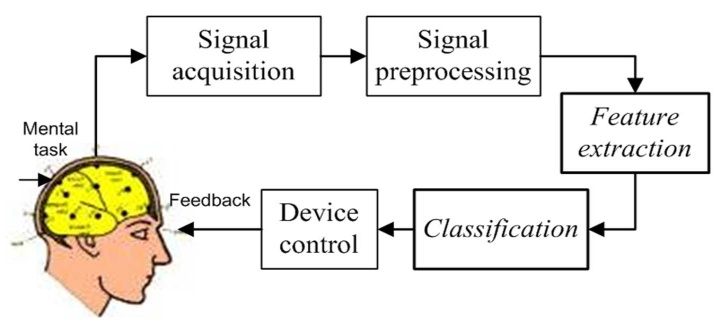
\includegraphics[width=0.9\textwidth]{bci.png}}
	\caption{Общая схема работы нейрокомпьютерных интерфейсов.}
	\label{bci}
	\end{figure}

	\subsection{Предобработка}
	\par Предобработка сигнала проводится с целью удаления артефактов (спонтанные сокращения мышц, моргание и т.п.), а также нейтрализации имеющихся шумовых компонент. Кроме того, зачастую интересующая информация содержится в определённом диапазоне частот, а остальные компоненты являются малоинформативными.
	\setcounter{pe}{0}
	\NepS {\bf Удаление постоянного амплитудного смещения}
	\par {\it Постоянное амплитудное смещение} (англ. {\it direct current offset}, {\it DC offset}, постоянное смещение потока) ~--- отклонение волновой формы относительно оси нулевого уровня сигнала. Амплитудное смещение, наблюдаемое в электроэнцефалограмме, может быть разложено на две основные составляющие: постоянное смещение, возникающее из-за технических особенностей передачи данных, и  смещение, возникающее из-за взаимодействия электрической цепи с потенциалом тела.\\
	\NepS {\bf Полосовая фильтрация}
	\par Как было упомянуто выше, в электроэнцефалограмме здорового человека выделяют несколько характерных составляющих электрических колебаний, называемых ритмами, различающихся частотным диапазоном. С целью выявления компонент, отвечающих соответствующим ритмам, применяются методы фильтрации в заданном диапазоне частот. Диапазон частот выбирается, исходя из априорной информации о ритмах.
	\par {\it Фильтрами нижних частот} (англ. {\it low-pass filter, LPF}) называется тип фильтров, эффективно пропускающих частотный спектр сигнала ниже некоторой частоты (т.н. {\it частоты среза}) и уменьшающих (подавляющих) частоты сигнала выше этой частоты. Степень подавления каждой частоты зависит от вида фильтра. {\it Фильтр верхних частот} (англ. {\it high-pass filter, HPF}), напротив, пропускает частоты выше частоты среза и подавляет низкие частоты.\\
	\NepS {\bf Робастное преобразование}
	\par Одним из эффективных методов снижения влияния артефактов, имеющих место в данных ЭЭГ, является робастное преобразование данных для каждого сенсора. Для каждого электрода вычисляются значения перцентилей среза (см. рис.~\ref{windsorization}), затем значения, лежащие ниже или выше полученных значений, замещаются соответствующими значениями.
	\newline

	\begin{figure}[h!]
	\center{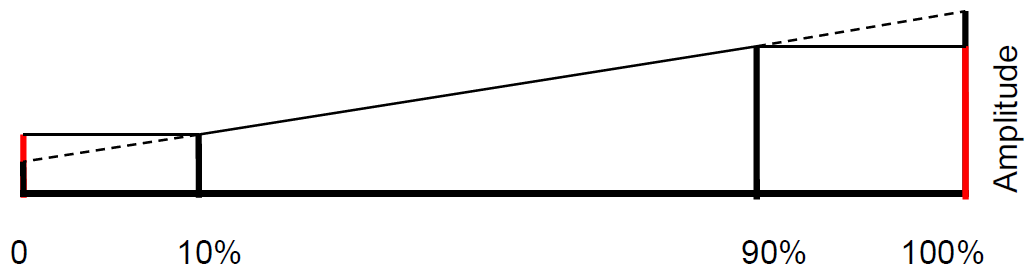
\includegraphics[width=0.9\textwidth]{windsorization.png}}
		\caption{Принцип работы робастного преобразования данных.}
	\label{windsorization}
	\end{figure}

	\NepS {\bf Отбор электродов}
	\par Современные электроэнцефалографы оснащены десятками электродов, однако информация, получаемая при помощи такого количества сенсоров, является избыточной. Кроме того, увеличение числа электродов ведёт к повышению стоимости устройства и времени на подготовку к использованию, что является недопустимым для электроэнцефалографов, разработанных для коммерческого использования. В связи с этим в современных исследованиях по тематике нейрокомпьютерных интерфейсов наиболее распространены два подхода к решению данной проблемы:
	\begin{enumerate}[1)]\itemsep-4pt
	\item выбор электродов с учётом априорных знаний о локализации компонент сигнала на скальпе;
	\item использование методов отбора признаков.
	\end{enumerate}

	\subsection{Построение признакового пространства}
	\par Применение классических методов распознавания в классе задач нейрокомпьютерных интерфейсов малоэффективно в силу множества причин, среди которых высокая степень зашумлённости данных, высокая размерность пространства, а также многомерность самих сигналов и т.п. В связи с этим этап построения признакового пространства является самым важным в процессе решения задачи. Проблема заключается в том, что не существует единого метода поиска нового признакового пространства. Каждый исследователь сталкивается с необходимостью поиска признакового пространства для эффективного решения конкретной поставленной задачи с использованием конкретного оборудования. \\
	\setcounter{pe}{0}
	\NepS {\bf Разделение источников вслепую}
	\par Семейство методов разделения источников вслепую (англ. {\it blind source separation}) основано на предположении о том, что регистрируемые сигналы для мультиканального устройства являются смесью сигналов из различных источников, и является попыткой выделить исходные источники, преобразуя зарегистрированные сигналы. Классическим примером задачи, иллюстрирующей функциональность данных методов, яволяется <<задача коктейльной вечеринки>> (англ. {\it cocktail party problem}). Предполагается, что фиксируемые сигналы $X(t) = [x_1(t), \dots, x_n(t)]$ с использованием $n$ сенсоров являются линейными комбинациями $p$ исходных сигналов $S(t) = [s_1(t), \dots, s_p(t)]$:
$$X(t) = AS(t),$$
	где $A \in \mathbb{R}^{n \times p}$ -- неизвестная <<смешивающая>> матрица. Отметим, что для успешного решения задачи необходимо выполнения условия $n \geqslant p.$ Затем метод разделения источников вслепую производит поиск соответствующей <<разделяющей>> матрицы $W$, наилучшим образом оценивающей исходные сигналы:
$$\widehat{S}(t) = WX(t),$$
	где $\widehat{S}(t)$ - оценка компонент источников $S(t)$. Кроме того, есть возможность оценки смешивающей матрицы $A$ и последующей реконструции исходных данных.
	\paragraph{Метод главных компонент.}
	\par Метод главных компонент (англ. {\it principal component analysis, PCA}) — метод поиска линейного преобразования данных путём максимизации дисперсии преобразованных данных. Задача может быть решена с использованием собственных векторов эмпирической матрицы ковариаций $X^TX$:
$$X^TX \alpha = \lambda \alpha,$$
	где $\alpha$ - собственный вектор матрицы, отвечающий собственному значению $\lambda$. Набор собственных векторов образует ортогональный базис, в котором представляются исходные данные. В случае отсортированных в порядке убывания собственных значений большая часть вариации данных будет сосредоточена в первых координатах, что позволяет перейти к пространству меньшей размерности.
	\paragraph{Метод независимых компонент.}
	\par Метод независимых компонент (англ. {\it independent component analysis, ICA}) -- метод, который может быть применен к произвольному набору случайных величин с целью нахождения линейного преобразования, максимизирующего статистическую независимость результирующих компонент. В то время как метод главных компонент опирается лишь на статистические моменты второго порядка, метод независимых компнент может быть назван его обобщением. В \cite{Cachenoura} данный метод определяется как оптимизационная задача минимизации совместной информации компонент источников. В упомянутом исследовании был представлен эффективный алгоритм вычисления негауссовости, напрямую связанной со статистической независимостью.
	\par При использовании в задачах классификации волн P300 метод независимых компонент показал способность изолировать данный тип волн в качестве компонент источников, упомянутых выше.
	\par Существует множество различных реализаций метода независимых компонент, отличающихся в том числе используемым определением независимости компонент источников. По результатам сравнения нескольких ICA алгоритмов \cite{Cachenoura}, используемых  в исследованиях нейрокомпьютерных интерфейсов, для применения в данной работе был выбран алгоритм {\it FastICA}~\cite{FastICA}, продемонстрировавший хорошие результаты и использующий коэффициент эксцесса в качестве меры негауссовости.
	\par Коэффициент эксцесса является мерой остроты пика распределения случайной величины и  определяется формулой 
	$$\gamma_2 = \frac{\mathbb{E} [(X - \mathbb{E} X)^4]}{(\mathbb{D} X)^2} - 3.$$
	Значение данного коэффициента позволяет проводить сравнение распределения некоторой случайной величины и нормального распределения, поскольку коэффициент эксцесса нормального распределения равняется нулю. Положительное значение коэффициента эксцесса означает, что большая часть дисперсии сигнала является результатом значимых, однако редко имеющих место отклонений, тем самым порождая распределение с <<тяжелыми>> хвостами. Алгоритм {\it FastICA} проводит поиск источников, отвечающих экстремуму коэффициента эксцесса.
	\newline
	
	\NepS {\bf Морфологические признаки}
	\par Морфологические признаки описывают изменения амплитуд нейрофизиологических сигналов, происходящих в течение определённого временного промежутка. Часто используемая стратегия разделения фоновой активности и волн P300 состоит в применении фильтра низких частот или фильтра с некоторой полосой пропускания с последующим возможным прореживанием сигнала, поскольку большая часть компоненты волны P300 сконцентрирована именно в области низких частот, а потому описанная процедура позволяет нейтрализовать влияние избыточной информации. Помимо прочего, это также ведёт к снижению размерности сигнала.
	\par Пусть имеется сигнал $s = [s_1, \dots, s_T].$ Для описания формы сигнала могут быть вычислены морфологические признаки, используемые отдельно или совместно с другими признаками. Некоторые из них перечислены ниже.
	\begin{itemize}
	\item 
	{\bf Амплитуда} -- максимальное значение сигнала: $\displaystyle s_{max} = \max_{t = 1, \dots, T} \{{s_t}\}$.
	\item
	{\bf Латентность} -- момент регистрации максимального значения сигнала для вызванных потенциалов: $\displaystyle t_{max} = \arg \max_{t=1, \dots, T} \{ s_t \}$, где $s$ регистрируется в течение фиксированного промежутка после выделения стимула.
	\item
	{\bf Отношение латентность/амплитуда}: $\displaystyle LAR = \frac{t_{max}}{s_{max}}$.
	\item
	{\bf Абсолютная амплитуда}: $\displaystyle AAMP = \left| s_{max} \right|$.
	\item
	{\bf Абсолютное отношение латентность/амплитуда}: $\displaystyle ALAR = \left| \frac{t_{max}}{s_{max}} \right|$.
	\item
	{\bf Положительная область} -- сумма положительных значений сигнала: \\ $\displaystyle PAR~=~\sum_{t = 1} ^ T \frac{s_t + |s_t|}{2}.$
	\item
	{\bf Отрицательная область} -- сумма отрицательных значений сигнала: \\$\displaystyle NAR~=~\sum_{t = 1} ^ T \frac{s_t - |s_t|}{2}.$
	\item
	{\bf Межпиковая разность}: $\displaystyle PP = s_{max} - s_{min},$ где $s_{max}$ и $s_{min}$ - максимальное и минимальное значения сигнала соответственно.
	\item
	{\bf Межпиковое расстояние}: $\displaystyle PPT = t_{max} - t_{min}.$
	\end{itemize}


	\NepS {\bf Преобразование Фурье}
	\par Зачастую анализ сигналов проводится при помощи разложения на <<базисные>> функции, каждая из которых отвечает некоторой частоте. Таким образом можно проанализировать степень выраженности колебаний некой частоты. В частности, преобразование Фурье использует в качестве базисных функций синусоиды. Для дискретных сигналов, имеющих место в задаче построения нейрокомпьютерного интерфейса, применяется дискретное преобразование Фурье (ДПФ).
	\par Пусть имеется дискретный сигнал $x = (\, x_0, \, \ldots, \, x_{N-1}\, )$. Тогда его можно представить в виде линейной комбинации дискретных синусоид следующего вида:
$$x_n = \sum_{k=0}^{\frac{N}{2}} C_k \cos{\frac{2 \pi k (n + \phi_k)}{N}}\, = \, \sum_{k=0}^{\frac{N}{2}} A_k \cos{\frac{2 \pi k n}{N}} + \sum_{k=0}^{\frac{N}{2}} B_k \sin{\frac{2 \pi k n}{N}}, \quad n = \overline{0, N-1}.$$
	Для каждого сигнала можно однозначно определить коэффициенты $A_k,\, B_k,$ называемые {\it спектром} сигнала. Получение коэффициентов при имеющемся сигнале называется {\it прямым преобразованием Фурье}, в то время как обратный процесс, синтез сигнала по имеющимся коэффициентам, называется {\it обратным преобразованием Фурье}. Наиболее часто используется {\it быстрое преобразование Фурье (БПФ)}, позволяющее выполнять преобразования значительно быстрее за счёт  наличия повторяющихся значений при вычислениях в силу периодичности функции синуса. 
	\par По аналогии можно произвести подобное разложение и для двумерного сигнала, при этом непосредственное вычисление двумерного ДПФ по полученным формулам требует огромных вычислительных затрат. Однако можно показать, что двумерное ДПФ обладает свойством сепарабельности, то есть его можно вычислить последовательно по двум измерениям. 
	\par Отметим также, что преобразование Фурье является чувствительным к шуму.

	\NepS {\bf Вейвлет-преобразование}
	\par Вейвлет-преобразование — интегральное преобразование, которое представляет собой свертку вейвлет-функции, обладающей рядом характерных свойств, с сигналом. По аналогии с преобразованием Фурье происходит некое разложение исходного сигнала. Для дискретных сигналов используется дискретное вейвлет-преобразование.
	\par Пусть имеется дискретный сигнал $x = (\, x_0, \, \ldots, \, x_{N-1}\, )$. Дискретное вейвлет-преобразование осуществляется путём применения набора фильтров. Сигнал подвергается действию фильтра низких частот с импульсным откликом $g$ и фильтра высоких частот с импульсным откликом $h$, в результате чего могут быть получены т.н. {\it коэффициенты аппроксимации} и {\it детализирующие коэффициенты} соответственно. После этого каждый из наборов коэффициентов прореживается в два раза. Кроме того, данное разложение может быть повторено с дальнейшим прореживанием коэффициентов после низкочастотной и высокочастотной фильтрации. Данный процесс может быть представлен в виде двоичного дерева, где листья и узлы соответствуют пространствам с различной частотно-временной локализацией. Схема действия одно- и трёхуровнего дискретного вейвлет-преобразования приведена на рис.~\ref{wavelet_scheme}.
	\par Многоуровневое дискретное вейвлет-преобразование может быть представлено в виде вычисления коэффициентов путём сдвига и масштабирвования т.н. {\it базового} вейвлета.

\begin{figure}[h!]
\begin{minipage}[h!]{1.0\linewidth}
\center{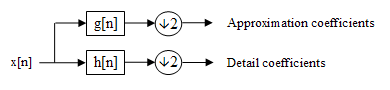
\includegraphics[width=0.6\linewidth]{wave1.png} \\ а)}
\end{minipage}
\begin{minipage}[h!]{1.0\linewidth}
\center{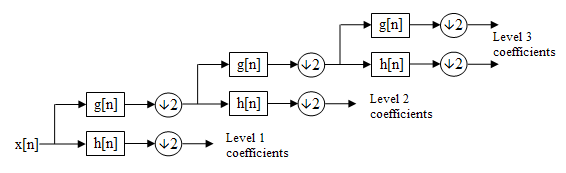
\includegraphics[width=0.8\linewidth]{wave2.png} \\ б)}
\end{minipage}
\caption{Схема действия одно- (а) и трёхуровнего дискретного вейвлет-преобразования.}
\label{wavelet_scheme}
\end{figure}
	\mbox{}\newline
	\NepS {\bf Общий пространственный фильтр}
	\par Общий пространственный фильтр (англ. {\it Common Spatial Pattern Filter, CSP}) реализует метод декомпозиции многоканального ЭЭГ сигнала, основанный на обучении по прецедентам.
	\par Рассматривается задача классификации многомерных сигналов на два класса. Целью метода является разложение исходного сигнала на аддитивные составляющие таким образом, чтобы максимизировать дисперсию первых компонент и минимизировать дисперсию последних для объектов первого класса и добиться обратной ситуации для объектов второго класса. Матрица декомпозиции может быть найдена в результате одновременной диагонализации выборочных матриц ковариации для каждого из классов. В результате может быть сформирован вектор характерных признаков путём соединения значений некоторого количества первых и последних компонент разложенного сигнала.
	\par Метод также может быть обобщён для применения к задачам с количеством классов, большим двух, путём разбиения исходной задачи на бинарные подзадачи с использованием схем <<один против одного>> или <<один против всех>>.

	\subsection{Классификация}
	\par После построения искомого признакового пространства алгоритм, используемый для классификации преобразованных объектов, играет не столь значительную роль. После предобработки и преобразования исходных данных проводится обучение классификатора, после чего обученный классификатор может принимать решение о наличии либо отсутствии волн P300 и, как следствие, о необходимости выполнять действие, предписанное стимулом. Наиболее часто в исследованиях по тематике {\it BCI} используются описанные ниже типы классификаторов. Более подробное описание данных алгоритмов может быть найдено в~\cite{Vorontsov}.
	\newline	\newline	\newline
	\setcounter{pe}{0}
	\NepS {\bf Байесовский классификатор}
	\par Байесовский классификатор — широкий класс алгоритмов классификации, основанный на принципе максимума апостериорной вероятности. Для классифицируемого объекта вычисляются функции правдоподобия каждого из классов, по ним вычисляются апостериорные вероятности классов. Объект относится к тому классу, для которого апостериорная вероятность максимальна.
	\par Байесовский подход к классификации основан на теореме, утверждающей, что если плотности распределения каждого из классов известны, то искомый алгоритм можно выписать в явном аналитическом виде. Более того, этот алгоритм оптимален, то есть обладает минимальной вероятностью ошибок.
	\par На практике плотности распределения классов, как правило, не известны. Их приходится оценивать (восстанавливать) по обучающей выборке. В результате байесовский алгоритм перестаёт быть оптимальным, так как восстановить плотность по выборке можно только с некоторой погрешностью. Зачастую в исследованиях по тематике создания нейрокомпьютерного интерфейса в качестве функции правдоподобия для объекта используется смесь нормальных распределений.\\
	\NepS {\bf Линейный дискриминант Фишера}
	\par Линейный дискриминант Фишера (ЛДФ) -- особый вариант байесовского классификатора. Рассмотрим задачу классификации на два класса. Предполагается, что обучающая выборка составлена таким образом, что классы распределены по нормальному закону, а матрицы ковариаций классов равны. Простота классификации линейным дискриминантом Фишера -- одно из достоинств алгоритма: в случае с двумя классами в двумерном признаковом пространстве разделяющей поверхностью будет прямая. Если классов больше двух, то разделяющая поверхность будет кусочно-лиинейной.
	\par Данный метод классификации не требует больших вычислительных затрат, а потому является распространённым в приложениях, функционирующих в режиме реального времени.\\
	\NepS {\bf Нейронные сети}
	\par Нейронные сети широко используются во многих приложениях, решающих задачу классификации, поскольку обладают гибкостью. Классическая модель нейронной сети состоит из узлов, называемых {\it нейронами}, и связей между ними, называемых {\it синапсами}, при этом узлы организованы в т.н. {\it слои}. Входной слой получает вектор описания объекта, подвергаемого классификации, выходной слой принимает итоговое решение о классификации данного объекта. Помимо двух упомянутых слоёв в нейронной сети также может присутствовать некоторое количество {\it скрытых} слоёв. Каждому из синапсов ставится в соответствие некоторое вещественное число, называемое {\it весом}, используемое при вычислении входных данных для следующего слоя нейронов. Каждому из нейронов ставится в соответствие некоторая {\it функция активации}, применяющаяся к сумме данных всех синапсов, оканчивающихся в данном нейроне, с целью получения выхода данного нейрона. 
	\par Задача обучения нейронной сети состоит в настройке весов синапсов, имеющих место в используемой модели. Одной из широко применяемых моделей нейронных сетей в задачах построения нейрокомпьютерных интерфейсов является сеть прямого распространения, обучаемая при помощи метода обратного распространения ошибки (англ. {\it backpropagation}).\\
	\NepS {\bf Метод опорных векторов}
	\par Метод опорных векторов (англ. {\it support vector machine, SVM}) — набор схожих алгоритмов обучения с учителем, принадлежащий к семейству линейных классификаторов. Особым свойством метода опорных векторов является непрерывное уменьшение эмпирической ошибки классификации и увеличение зазора, поэтому метод также известен как метод классификатора с максимальным зазором. Кроме того, на положение разделяющей гиперплоскости в действительности оказывает влияние небольшая часть объектов обучающей выборки. Метод также обобщается на случай нелинейной разделяющей поверхности.
	\par Зачастую используется в исследованиях по тематике {\it BCI} в силу сводимости к задаче квадратичного программирования и последующей эффективности вычислений.\\
	\NepS {\bf Метод k ближайших соседей}
	\par Метод $k$ ближайших соседей (англ. {\it k-nearest neighbor algorithm, kNN}) — метод автоматической классификации объектов. Основным принципом метода ближайших соседей является то, что объект присваивается тому классу, который является наиболее распространённым среди соседей данного элемента. Соседи выбираются из обучающей выборки, и, исходя из ключевого для данного метода значения $k$, вычисляется наиболее распространённый среди них класс.
	\par Таким образом, если в процессе формирования признакового пространства удалось некоторым образом локализовать объекты каждого из классов в некоторой области пространства, данный метод может быть использован для классификации преобразованных объектов. Кроме того, среди достоинств данного метода следует упомянуть вычислительную простоту, что делает его простым для использования в приложениях, функционирующих в режиме реального времени.

	\subsection{Критерий качества}
	\par Важным аспектом всякой системы {\it BCI} является достигаемая скорость коммуникации. В системах, основанных на распознавании волн P300, данная характеристика зависит от межстимульного интервала, количества различных стимулов, качества работы классификаторов. Чтобы проследить зависимость от перечисленных факторов, будем использовать в качестве метрики для оценивания скорости коммуникации скорость передачи информации (битрейт). Битрейт оценивает количество бит, передаваемых испытуемым системе в единицу времени. Данная характеристика широко используется для оценки работы нейрокомпьютерных интерфейсов, в том числе и не основанных на волнах P300.
	\par Определим матрицу ошибок для задачи классификации на два класса, разделив эпохи для целевых и нецелевых стимулов на верно и неверно классифицированные:
	\begin{itemize}\itemsep-4pt
	\item
	$a$ -- количество {\bf верно} классифицированных {\bf нецелевых} эпох;
	\item
	$b$ -- количество {\bf неверно} классифицированных {\bf нецелевых} эпох;
	\item
	$c$ -- количество {\bf неверно} классифицированных {\bf целевых} эпох;
	\item
	$d$ -- количество {\bf верно} классифицированных {\bf целевых} эпох.
	\end{itemize}

\begin{table}[h]
\centering
\begin{tabular}{|ll|l|l|}
\hline
 &  & \multicolumn{2}{l|}{Предсказанный тип стимула} \\ \cline{3-4} 
 &  & Нецелевой & Целевой \\ \hline
\multicolumn{1}{|l|}{\multirow{2}{*}{\begin{tabular}[c]{@{}l@{}}Реальный тип\\ стимула\end{tabular}}} & Нецелевой & $a$ & $b$ \\ \cline{2-4} 
\multicolumn{1}{|l|}{} & Целевой & $c$ & $d$ \\ \hline
\end{tabular}
\caption{Матрица ошибок для задачи распознавания волн P300.}
\label{confusion}
\end{table}

	Таким образом, можно составить таблицу~\ref{confusion}. {\it Чувствительностью} (англ. {\it true positive rate, TPR}) называется доля верно классифицированных целевых эпох, {\it специфичностью} (англ. {\it false positive rate, FPR}) -- доля неверно классифицированных нецелевых эпох. Данные величины могут быть вычислены по следующим формулам:
$$TPR = \frac{d}{c+d},$$
$$FPR = \frac{b}{a+b}.$$
	Положим $n_1 = c+d$ - количество целевых эпох, $n_2 = a+b$ - количество нецелевых эпох. Тогда битрейт может быть вычислен по следующей формуле:
$$BR = \frac{d}{n_1 + n_2} \times \frac{60}{ISI} \times \log_2 (N_{st}),$$
где $ISI$ - межстимульный интервал (сек), т.е. промежуток времени между демонстрацией двух последовательных стимулов, $N_{st}$ - количество различных визуальных стимулов, используемых в эксперименте.
	\par Кроме указанных величин, {\it точность} системы может быть вычислена по формуле:
	$$Accuracy \% = \frac{a+d}{a+b+c+d} \times 100 \%.$$
	\par Указанные величины широко используются в литературе по исследуемой тематике для оценки качества функционирования системы. В связи с этим будем использовать совокупность указанных характеристик для оценки эффективности интерфейса.
\newpage

\section{Проведение эксперимента}
\subsection{Парадигма эксперимента}
	\par Как правило, в исследованиях на основе визуальных стимулов используется следующая схема получения данных:
	\begin{itemize}
	\item
	Испытуемому в течение $t_1$ секунд демонстрируется визуальный стимул либо ментальное задание, которое предстоит выполнить. Значение $t_1$ варьируется для различных типов исследований.
	\item
	В течение $t_2$ секунд испытуемый сосредотачивает внимание на визуальном стимуле либо выполняет указанное ментальное задание. Кроме того, в процессе этого действия происходит запись данных. Значение $t_2$ варьируется для различных типов исследований.
	\item
	Визуальный стимул перестаёт демонстрироваться испытуемому, проводится краткая пауза для восстановления расслабленного состояния и подготовки к следующей итерации.
	\end{itemize}

	\par После изучения материалов по исследуемой тематике и различных видов парадигм, используемых для тестирования применимости разработанных систем управления, было принято решение провести две серии эксериментов, использующих различные виды визуальных стимулов. 
	\par Получение данных для каждого из двух испытуемых производилось следующим образом. Испытуемый располагался лицом к монитору компьютера с устройством {\it Emotiv EPOC}, расположенным на голове. На экране монитора было изображено квадратное поле, разбитое на 100 равных квадратов прямыми, параллельными его сторонам, путём деления каждой стороны на 10 равных отрезков. Каждый из квадратов является возможным положением курсора на экране компьютера. Целью испытуемого являлось управление курсором в виде голубого квадрата, расположенного на экране компьютера, от начального до обозначенного конечного положения путем перемещения сначала по горизонтали, а затем -- по вертикали. Четыре визуальных стимула выделялись на экране последовательно случайным образом, в каждый момент времени было выделено не более одного визуального стимула. В первой серии экспериментов в качестве визуальных стимулов выступали изображения стрелок, отвечающих четырём возможным направлениям движения курсора (вверх, вниз, влево, вправо); во второй серии экспериментов использовались текстовые надписи, описывающие одно из указанных направлений движения. Внешний вид используемого поля и визуальных стимулов в двух сериях экспериментов изображен на рис.~\ref{field}. Испытуемому требовалось сконцентрировать внимание на стимуле, отвечающем желаемому направлению движения (целевом стимуле с вероятностью появления 25\%), и игнорировать остальные стимулы, отвечающие нежелательным направлениям движения курсора (нецелевые стимулы с вероятностью появления 75\%).

\begin{figure}[h!]
\begin{minipage}[h!]{0.49\linewidth}
\center{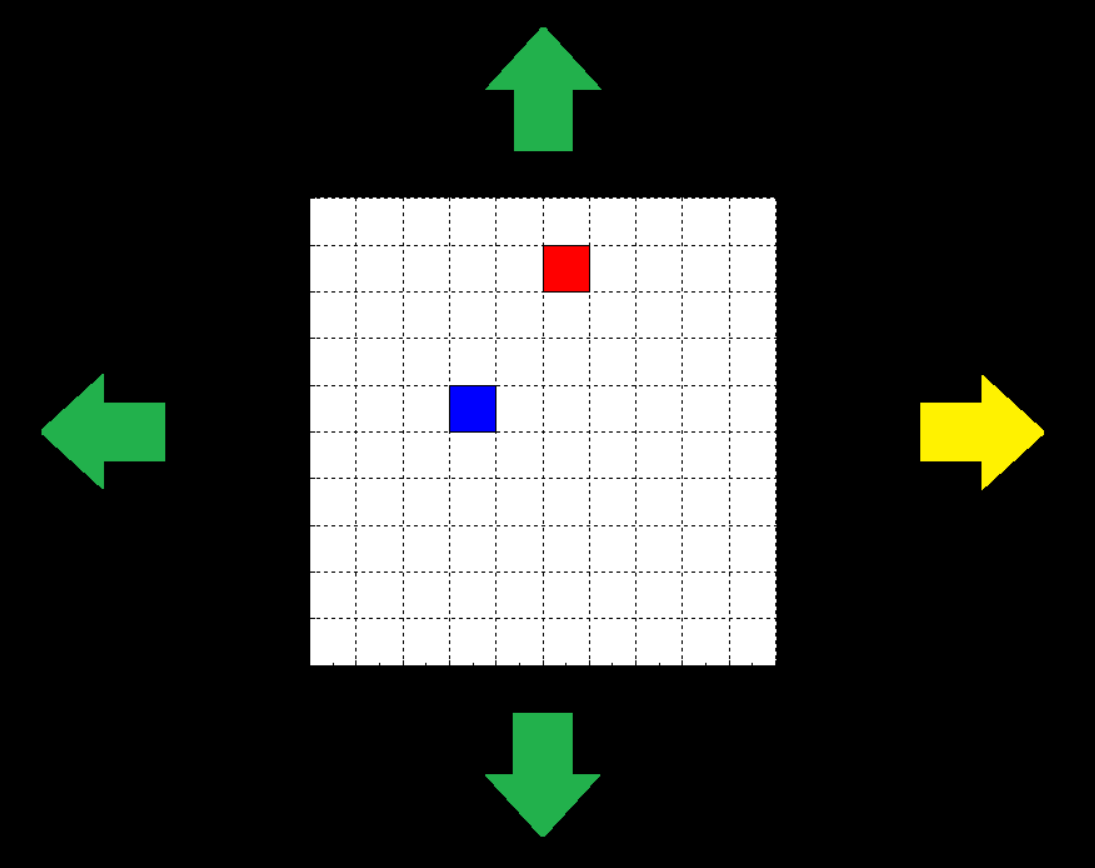
\includegraphics[width=1\linewidth]{stimuli1.png} \\ а)}
\end{minipage}
\hfill
\begin{minipage}[h!]{0.49\linewidth}
\center{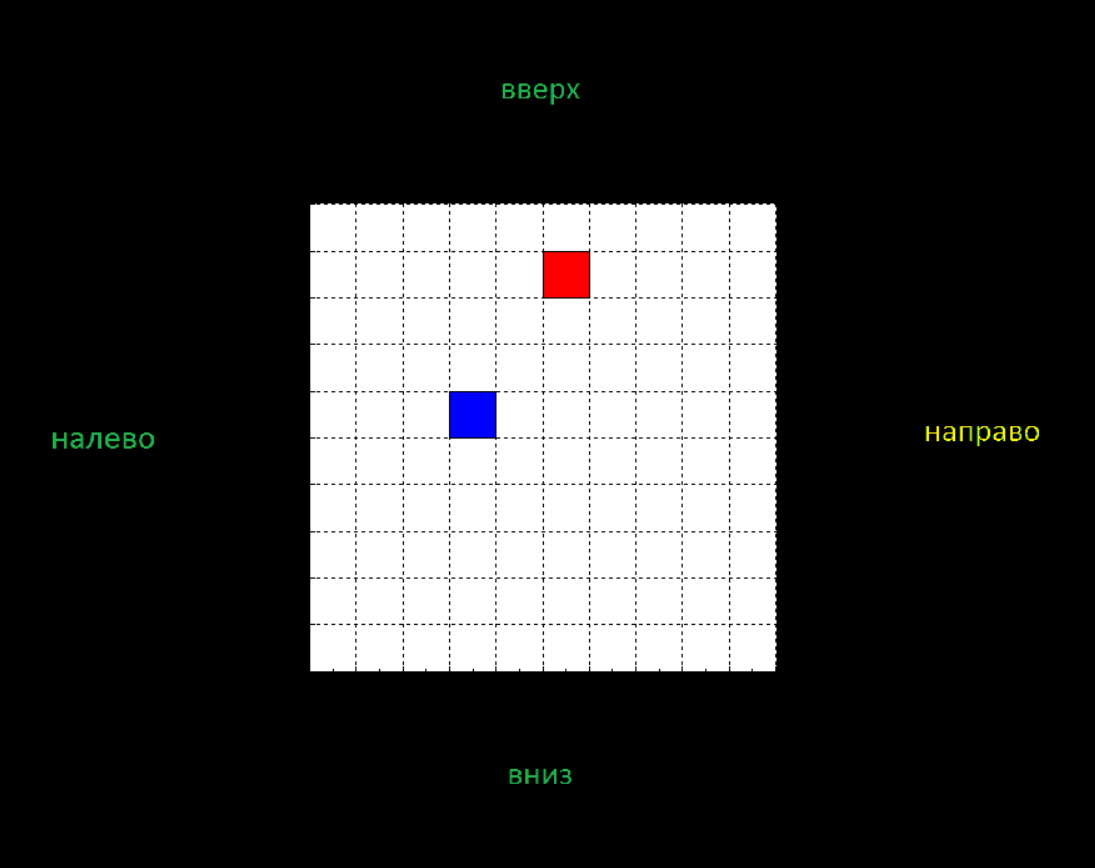
\includegraphics[width=1\linewidth]{stimuli2.png} \\ б)}
\end{minipage}
\caption{Поле и визуальные стимулы, изображённые на экране компьютера в процессе проведения серий экспериментов с различными видами стимулов.}
\label{field}
\end{figure}

	\par {\it Пробой} назовем последовательность из выделения некоторого визуального стимула в течение 250 мс, а также последующие 1250 мс, необходимые для обработки, классификации данных, генерации команды и выполнения перемещения курсора. Межстимульный интервал при проведении эксперимента равнялся 2500 мс, включая время, необходимое на обработку и классификацию данных. Назовём {\it сессией} последовательность проб, предпринятых для достижения курсором целевого положения.
	\par Запись ЭЭГ осуществлялась с частотой дискретизации 128 Гц (с внутренней частотой дискретизации устройства 2048 Гц и последующей первичной обработкой) при помощи устройства {\it Emotiv EPOC}. При записи данных устройство находилось в двух различных положениях: положение по умолчанию и инверсированное положение. В положении по умолчанию были использованы данные 10 сенсоров (F3, FC5, T7, P7, O1, O2, P8, T8, FC6, и F4), поскольку данное подмножество обеспечивает наилучшую нейтрализацию компонент, не отвечающих за волны P300, а также включает сенсоры O1, O2, при помощи которых могут быть зафиксированы некоторые из компонент волн P300~\cite{ensemble}. В инверсированном положении были использованы данные 8 сенсоров (FC6, F4, P8, AF4, AF3, F3, P7 и FC5), поскольку они покрывают центральную часть скальпа, которая считается областью, участвующей в генерации волн P300. Положения указанных сенсоров на голове человека изображены на рис.~\ref{position}.

\begin{figure}[h!]
\begin{minipage}[h!]{0.48\linewidth}
\center{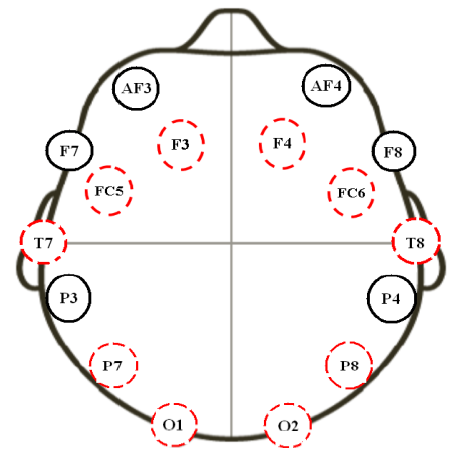
\includegraphics[width=1\linewidth]{default.png} \\ а)}
\end{minipage}
\hfill
\begin{minipage}[h!]{0.5\linewidth}
\center{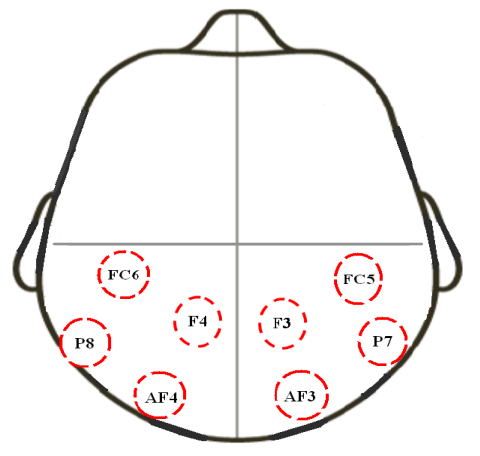
\includegraphics[width=1\linewidth]{inverse.png} \\ б)}
\end{minipage}
\caption{Положения сенсоров для положения устройства по умолчанию (а) и инверсированного положения (б).}
\label{position}
\end{figure}


\subsection{Схема эксперимента}
	\par Наиболее распространённая схема эксперимента в исследованиях нейрокомпьютерных интерфейсов, основанных на выявлении волн P300, предполагает, что ответ на целевой стимул не зависит от конкретного стимула, в связи с этим классификация является эффективным методом распознавания целевых и нецелевых стимулов. Тем не менее, некоторые исследования, в частности \cite{ensemble}, описывают применение отдельных классификаторов и демонстрируют, что таким образом производительность системы может быть повышена. В связи с этим было решено применить оба подхода и сравнить полученные результаты.
	\par Схема эксперимента для каждого испытуемого состояла из двух частей: предобучение и тестирование в режиме реального времени. В процессе предобучения пользователю необходимо произвести предписанную последовательность действий, описанную ниже, позволяющую собрать некоторое количество данных, используемых для обучения классификатора. В процессе тестирования в режиме реального времени пользователю необходимо производить похожую процедуру, однако полученные данные для каждого из стимулов обрабатываются и классифицируются при помощи предобученного классификатора в тот же момент времени, а также принимается решение о наличии или отсутствии P300-волн и, соответственно, необходимости перемещения курсора в соответствующем направлении.
	\par Для функционирования обоих подходов необходимо проведение процедуры предобучения отдельно для каждого испытуемого (в силу физиологических различий, ненадёжной фиксации устройства на голове человека, изменения потенциала тела человека с течением времени и т.д.). Предобучение проводится по следующей схеме:
	\begin{itemize} 
	\item
	Испытуемый концентрирует внимание на фиксированном визуальном стимуле в течение $N$ раундов. Было проведено несколько серий экспериментов для различных значений $N$, в частности $N = 10, 15, 20, 30.$
	\item
	Раунд представляет из себя следующую последовательность действий. В течение раунда каждый из четырех визуальных стимулов, отвечающих возможным направлениям движения курсора, выделяется в течение 250 мс, затем следует период ожидания продолжительностью 2250 мс. 
	\item
	После $N$ раундов процесс останавливается на 10 секунд для восстановления расслабленного состояния и подготовки к следующей серии раундов, а затем проводятся раунды для следующего визуального стимула до тех пор, пока не состоялись раунды для всех видов стимулов.
	\item
	Таким образом, обучающая сессия состоит из $4N$ раундов записи ЭЭГ, содержащих $4N$ эпох целевых данных и $12N$ эпох нецелевых данных, где {\it эпохой} мы будем называть промежуток времени, содержащий выделение одного из визуальных стимулов и последующий период ожидания вплоть до выделения последующего визуального стимула.
	\item
	Кроме того, также проводится $N$ эпох для записи данных, отвечающих спокойному состоянию испытуемого, т.е. испытуемый расслаблен, а визуальные стимулы не выделяются.
	\item
	Таким образом, количество нецелевых эпох составляет $13N$. 75\% имеющихся данных используются для обучения классификатора (машины опорных векторов и нейронной сети) для разделения целевых и нецелевых данных. Остальные 25\% данных используются для настройки параметров классификатора в процессе обучения.
	\end{itemize}
	\par Для схемы с использованием отдельных классификаторов используется аналогичный сценарий, однако число раундов для каждого направления удваивается.

\newpage
\section{Предлагаемый подход}
\subsection{Предобработка}
	\par Перед обучением классификатора данные были подвергнуты предобработке. Последовательность действий, применённых к данным, описана ниже. 

	\paragraph{Центрирование данных.}
	\par В первую очередь все данные, полученные с каждого электрода, были центрированы с целью нейтрализации постоянного амплитудного смещения. Затем среднее значение сигналов, полученных с электродов сравнения, было использовано для референциального монтажа данных. В положении устройства по умолчанию в качестве электродов сравнения были использованы позиции AF3 и AF4, в инверсированном - O1 и O2.
	\paragraph{Выделение отдельных проб.}
	\par После этого из полученных данных были выделены отдельные пробы продолжительностью 1500 мс. Начало пробы совпадало с началом выделения визуального стимула на экране компьютера, конец пробы приходился на момент через 1500 мс после начала выделения стимула (250 мс выделения визуального стимула и 1250 мс ожидания). Таким образом, для дальнейшей обработки и определения наличия волн P300 имеются данные, представленные в виде потенциалов, зарегистрированных для 192 моментов времени для каждого из сенсоров после выделения каждого из визуальных стимулов.
	\paragraph{Фильтрация.}
	\par Были проведены эксперименты с использованием различных типов цифровых фильтров для обработки полученных сигналов, в частности, полосно-пропускного фильтра Чебышева 4-го порядка 1-го типа, фильтра Баттерворта и эллиптического полосно-пропускной фильтра с полосой пропускания 0.16--43 Гц.
	\paragraph{Мeтод независимых компонент.}
	\par К данным ЭЭГ, подвергнутым фильтрации, был применен метод независимых компонент для извлечения независимых источников. Была использована реализация алгоритма {\it FastICA} для {\tt MATLAB}. Описание алгоритма было представлено в предыдущих разделах. Более подробно алгоритм описан в \cite{FastICA}.

	\subsection{Отбор признаков}
	\par В исследовании \cite{Piccione} был применен метод с использованием нечетких регуляторов (англ. {\it fuzzy control method}) для отбора признаков, наиболее похожих на волны P300, для дальнейшей классификации. Другие исследования используют неавтоматический метод отбора признаков. Поскольку в данной работе используется коммерческое {\it BCI}-устройство с высоким уровнем шума в получаемых данных, нет возможности ожидать наличия среди полученных независимых компонент наличие близкой к P300-волне, наподобие полученных в исследовании \cite{Piccione}. Кроме того, данный метод существенно увеличивает время обработки данных. В исследовании \cite{James} показано, что результирующие компоненты ICA, отличные от P300-волн, практически неотличимы для целевых и нецелевых проб, поскольку они являются компонентами одних и тех же источников артефактов в одинаковых условиях. Для первого подхода к компонентам, полученным при помощи метода независимых компонент, применяется дискретное вейвлет-преобразование 3-го порядка, где коэффициенты аппроксимации представляют собой  энергию сигнала в полосе P300-волн, включающих энергию сигнала в дельта-, тета- и части альфа-ритмов, как показано в некоторых исследованиях~\cite{alco}. Для второго подхода преобразование применяется непосредственно к данным ЭЭГ. Для обоих подходов был использован вейвлет Добеши, поскольку он широко распространён в литературе для подобных целей. Результирующие коэффициенты аппроксимации были использованы в качестве признаков и были конкатенированы в единые вектора. Результирующая размерность признакового представления объектов равнялась $N_e \times N_f,$ где $N_e$ -- количество сенсоров, $N_f$ -- количество признаков в одной пробе. Кроме аппроксимирующих коэффициентов, были также использованы описанные в предыдущих разделах морфологические признаки. С учётом продолжительности проб и типа применяемого дискретного вейвлет-преобразования, получаем $N_f = 18 + 9 = 27.$ С учётом выбора одного из указанных подмножеств электродов имеем $N_e = 8$ или $N_e = 10.$
	\par Далее отобранные признаки подвергались стандартизации, т.е. преобразованию, обеспечивающему нулевое среднее значение каждого признака и единичную матрицу ковариаций. Нормировочные константы вычисляются для каждого сенсора с учётом всех имеющихся в обучающей выборке данных, а затем также применялись к отложенной выборке. Отметим, что стандартизации отдельных проб без учёта остальной информации может уничтожить важную информацию об амплитуде имеющихся волн P300, в связи с этим необходимо проведение данной процедуры для всех зарегистрированных проб.

\subsection{Классификация}
	\par После предобработки и отбора признаков, наиболее вероятно характеризующих наличие либо отсутствие волны P300, проводились обучение и  настройка параметров классификатора. Как было упомянуто выше, данные центрированы и имеют единичную матрицу ковариаций. В качестве классификаторов были использованы нейронная сеть и машина опорных векторов.
	\par В качестве нейронной сети применялась нейронная сеть прямого распространения с одним скрытым слоем. Структура подобного классификатора изображена на рис.~\ref{nn}. Отметим, что распределение данных, получаемых каждым из нейронов входного слоя сети, осуществлялось между всеми нейронами скрытого слоя. В качестве функций активации для нейронов скрытого и выходного слоев была использована функция гиперболического тангенса в соответствии с рекомендациями~\cite{activation}. Поскольку метки классов соответствовали наличию и отсутствию волн P300, полученное итоговое значение являлось оценкой вероятности наличия волн данного типа. В соответствии с рекомендациями~\cite{neu_net} считалось, что итоговое значение, превышающее 0.76, свидетельствовало о наличии волн P300, иное значение -- об их отсутствии. Для обучения нейронной сети применялся метод обратного распространения ошибки.
	\begin{figure}[h!]
	\center{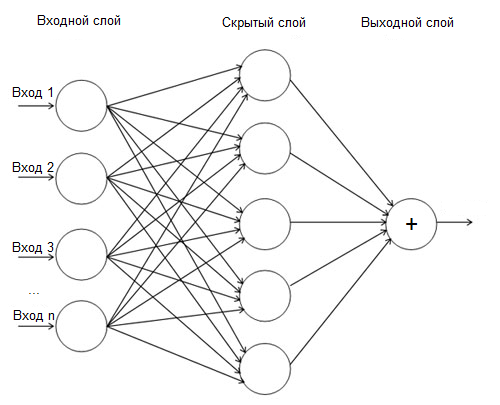
\includegraphics[width=1.0\textwidth]{network.png}}
		\caption{Структура используемой модели нейронной сети.}
	\label{nn}
	\end{figure}

	\par Кроме того, была использована реализация машины опорных векторов в библиотеке {\it LibSVM}. Для алгоритма с единым классификатором было использовано квадратичное ядро, в то время как для алгоритма с отдельными классификаторами была использована линейная версия {\it SVM}. Значение гиперпараметра $C$ настраивалось при помощи отложенной выборки.
	\par Для подхода с применением единого классификатора, обучающая выборка состояла из $4N$ целевых и $13N$ нецелевых эпох. В связи с высоким уровнем шума в данных было проведено усреднение по наборам из пяти эпох. Как было упомянуто выше, случайно выбранные 75\% полученных объектов были использованы для обучения классификатора, в то время как оставшиеся 25\% были использованы для настройки параметров.
	\par Для подхода, использующего отдельные классификаторы, были обучены четыре различных машины опорных векторов, отвечающих различным визуальным стимулам. В данном случае для каждого из классификаторов были доступны $N$ целевых и $4N$ нецелевых эпох, а усреднение проводилось по наборам из 3 эпох.

\subsection{Тестирование}
	\par После обучения классификатора необходим запуск процесса тестирования в режиме реального времени вручную. В течение этого времени ведётся запись данных ЭЭГ, при этом стимулы выделяются в случайном порядке в течение 250 мс с последующей паузой в течение 1250 мс. Данные, полученные в течение этого времени, подвергаются описанной процедуре предобработки и выделения признаков и дальнейшей классификации при помощи обученного классификатора. В случае принятия решения о наличии компоненты волн P300 курсор перемещается в соответствующем направлении, в случае противоположного решения -- процесс продолжается без перемещения курсора.

\newpage

\section{Результаты}
	\subsection{Результаты с положением устройства по умолчанию}
	\par Как было упомянуто выше, при расположении устройства в позиции по умолчанию малое число электродов покрывают часть скальпа, отвечающую за генерацию волн P300. В таком положении наибольшее влияние данного эффекта может быть замечено только на данных, регистрируемых при помощи сенсоров O1 и O2. В связи с этим результаты экспериментов, отображённые в таблицах~\ref{default_res_unite} и ~\ref{default_res_ens}, демонстрируют неприемлемо низкие уровни точности классификации и чувствительности, а также недопустимо высокий уровень специфичности по сравнению с результатами, полученными для инверсированного положения.

\begin{table}[h]
\centering
\begin{tabular}{|c|c|c|c|c|}
\hline
\begin{tabular}[c]{@{}c@{}}Количество раундов \\ $N$\end{tabular} & \begin{tabular}[c]{@{}c@{}}Чувствительность \\ (TPR)\end{tabular} & \begin{tabular}[c]{@{}c@{}}Специфичность \\ (FPR)\end{tabular} & Битрейт & Точность \\ \hline
10 & 24.53\% & 43.61\% & 1.15 & 45\% \\
15 & 26.13\% & 42.77\% & 1.22 & 47\% \\
20 & 27.7\% & 41.3\% & 1.23 & 48\% \\
30 & 28.4\% & 40.76\% & 1.24 &  50\% \\ \hline
\end{tabular}
\caption{Результаты применения подхода с единым классификатором для положения устройства по умолчанию.}
\label{default_res_unite}
\end{table}

\begin{table}[h]
\centering
\begin{tabular}{|c|c|c|c|c|}
\hline
\begin{tabular}[c]{@{}c@{}}Количество раундов \\ $N$\end{tabular} & \begin{tabular}[c]{@{}c@{}}Чувствительность \\ (TPR)\end{tabular} & \begin{tabular}[c]{@{}c@{}}Специфичность \\ (FPR)\end{tabular} & Битрейт & Точность \\ \hline
10 & 24.85\% & 43.24\% & 1.16 & 46\% \\
15 & 25.13\% & 42.83\% & 1.19 & 47\% \\
20 & 27.43\% & 41.72\% & 1.22 & 48\% \\
30 & 29.12\% & 40.12\% & 1.25 &  51\% \\ \hline
\end{tabular}
\caption{Результаты применения подхода с отдельными классификаторами для положения устройства по умолчанию.}
\label{default_res_ens}
\end{table}


	\subsection{Результаты с инверсированным положением устройства}
	\par Было проведено несколько серий экспериментов с использованием различных парадигм. В таблицах~\ref{reverse_res_unite} и~\ref{reverse_res_ens} отображены наилучшие полученные результаты.
\begin{table}[h]
\centering
\begin{tabular}{|c|c|c|c|c|}
\hline
\begin{tabular}[c]{@{}c@{}}Количество раундов \\ $N$\end{tabular} & \begin{tabular}[c]{@{}c@{}}Чувствительность \\ (TPR)\end{tabular} & \begin{tabular}[c]{@{}c@{}}Специфичность \\ (FPR)\end{tabular} & Битрейт & Точность \\ \hline
10 & 41.17\% & 34.2\% & 4.61 & 58\% \\
15 & 42.11\% & 33.89\% & 4.88 & 59\% \\
20 & 42.96\% & 33.02\% & 4.92 & 59\% \\
30 & 43.34\% & 32.74\% & 4.95 &  60\% \\ \hline
\end{tabular}
\caption{Результаты применения подхода с единым классификатором для инверсированного положения устройства.}
\label{reverse_res_unite}
\end{table}

\begin{table}[h]
\centering
\begin{tabular}{|c|c|c|c|c|}
\hline
\begin{tabular}[c]{@{}c@{}}Количество раундов \\ $N$\end{tabular} & \begin{tabular}[c]{@{}c@{}}Чувствительность \\ (TPR)\end{tabular} & \begin{tabular}[c]{@{}c@{}}Специфичность \\ (FPR)\end{tabular} & Битрейт & Точность \\ \hline
10 & 43.21\% & 30.24\% & 5.02 & 61\% \\
15 & 44.12\% & 29.87\% & 5.07 & 62\% \\
20 & 44.89\% & 29.91\% & 5.08 & 62\% \\
30 & 45.1\% & 28.34\% & 5.12 &  64\% \\ \hline
\end{tabular}
\caption{Результаты применения подхода с отдельными классификаторами для инверсированного положения устройства.}
\label{reverse_res_ens}
\end{table}

\subsection{Обсуждение и~выводы}
	\par Полученные результаты для системы с инверсированным положением устройства демонстрируют, что точность классификации предложенного подхода сравнима с существующими на данный момент исследованиями в данной области, использующими схожее оборудование и условия проведения экспериментов. В частности, в \cite{rhyme} была достигнута точность 60\% выявления волн P300 при использовании устройства {\it Emotiv EPOC.}
	\par Для испытуемых значение чувствительности оказалось довольно низким. Таким образом, система распознавала приблизительную предполагаемую траекторию движения курсора, однако для распознавания непосредственно команды необходимо было ожидание в течение нескольких проб, как следствие, наблюдалось падение производительности системы. Тем не менее, приемлемое значение точности может быть достигнуто при низком значении специфичности. Высокое же значение данной характеристики дезориентирует пользователя и может привести к невозможности дальнейшего управления курсором, поскольку траектория в таких случаях радикально отличается от предполагаемой пользователем. Отметим, что полученные значения специфичности сравнимы в результатами, полученными в \cite{Kanoh}. Предложенный в данной работе метод позволяет добиться лучших результатов по сравнению с подходом, предложенным в исследовании~\cite{pseudo}, при использовании {\it Emotiv EPOC}.
	\par Кроме того, в результате экспериментов было отмечено, что использование изображений стрелок в качестве визуальных стимулов ведёт к лучшим результатам, нежели изображений надписей.
	\par Наилучший результат был получен при применении подхода, использующего отдельные классификаторы для различных типов стимулов. Тем не менее, полученные результаты не свидетельствуют о том, что использование подхода отдельных классификаторов гарантирует лучший результат, нежели использование подхода с единым классификатором.
	\par Низкое значение точности полученной системы может быть результатом различных причин, среди которых следующие:
	\paragraph{Расположение сенсоров.}
	\par В инверсированном положении расположение электродов было приблизительным и, поскольку устройство было разработано для эксплуатации в позиции по умолчанию, некоторые из сенсоров ненадёжно крепились к голове испытуемого, не обеспечивая должного качества регистрируемого сигнала. Кроме того, изменились также и положения опорных электродов, тем самым повлияв на внутреннюю обработку получаемых данных в устройстве.
	\paragraph{Количество сенсоров.}
	\par Как было упомянуто выше, в положении устройства по умолчанию сенсоры не покрывают часть скальпа, отвечающую за генерацию волн P300. В инверсированном положении приблизительно не более шести электродов расположены в данной области, и, тем не менее, ни один из них не расположен в области, наиболее активно отвечающей за данный процесс.
	\paragraph{Отношение сигнал-шум.}
	\par Поскольку устройство было разработано для развлекательных целей, нет возможности гарантировать должное качество изготовления его деталей и, тем самым, качества снимаемого сигнала.

\newpage
\section{Заключение}
	\par В рамках настоящей дипломной работы были изучены существующие подходы к решению задач построения нейрокомпьютерных интерфейсов. Был предложен метод построения нейрокомпьютерного интерфейса для управления динамическим объектом, а также было проведено сравнение с аналогичными исследованиями последних лет.
	\par В ходе данной работы были получены следующие основные результаты:
	\begin{itemize}\itemsep0pt
		\item
		Предложен метод классификации сигналов головного мозга в задаче управления курсором на экране компьютера с использованием общедоступного устройства {\it Emotiv EPOC}.
		\item
		Предложенный метод был протестирован при помощи программной реализации в системе MATLAB.
		\item
		Результаты работы описанного подхода не уступают существующим на сегодняшний день методам решения данной задачи с использованием схожего оборудования. Сделанные выводы изложены в работе.
	\end{itemize}\par


\newpage

\renewcommand{\bibname}{Список литературы}
\addcontentsline{toc}{section}{\bibname}


\def\BibUrl#1.{}\def\BibAnnote#1.{}
%\def\BibUrl#1{\\{\footnotesize\tt\def~{\char126} http://#1}}
\bibliographystyle{plain}

\begin{thebibliography}{1}

\bibitem{Farwell_Donchin}
{\it Farwell~L.A., Donchin~E.} Talking off the top of your head: toward a mental prothesis utilizing event-related brain potentials. // Electroencephalography \& Clinical Neurophysiology, Vol. 70, Issue 6, pp. 510-523, 1988.

\bibitem{P300_first}
{\it Sutton~S., Braren~M., Zubin~J., John~E.R.} Evoked-potential correlates of stimulus uncertainty. // Science, Vol. 150,  Issue 700, pp. 1187-1188, 1965.

\bibitem{Cachenoura}
{\it Kachenoura~A., Albera~L., Senhadji~L., Comon~P.} ICA: A Potential Tool for BCI Systems. // Signal Processing Magazine, IEEE, Vol. 25, Issue 1, pp. 57-68, 2008.

\bibitem{ensemble}
{\it Rakotomamonjy~A., Guigue~V.} BCI Competition III: Dataset II- Ensemble of SVMs for BCI P300 Speller. // Biomedical Engineering, IEEE Transactions, Vol. 55, Issue 3, pp. 1147-1154, 2005.

\bibitem{FastICA}
\emph{The FastICA algorithm package for MATLAB}.
[HTML] (http://research.ics.aalto.fi/ica/fastica/).

\bibitem{Piccione}
{\it Piccione~F., Giorgi~F., Tonin~P., Priftis~K., Giove~S., Silvoni~S., Palmas~G., Beverina~F.} P300-based brain computer interface: reliability and performance in healthy and paralysed participants. // Clin Neurophysiol, Vol. 117, Issue 3, pp. 531-537, 2006.

\bibitem{James}
{\it Wang~S., James~C.J.} Enhancing evoked responses for BCI through advanced ICA techniques. // International Conference on Advances in Medical, Signal and Information Processing, pp. 1--4, 2006.

\bibitem{rhyme}
{\it Ramírez-Cortes~J.M., Alarcon-Aquino~V., Rosas-Cholula~G., Gomez-Gil~P., Escamilla-Ambrosio~J.} P-300 Rhythm Detection Using ANFIS Algorithm and Wavelet Feature Extraction in EEG Signals. // Proceedings of the World Congress on Engineering and Computer Science, Vol. 1,  pp. 963-968, 2010.

\bibitem{Kanoh}
{\it Kanoh S., Miyamoto K., Yoshinobu T.} A P300-based BCI System for Controlling Computer Cursor Movement. // Conf Proc IEEE Eng Med Biol Soc., 2011.

\bibitem{system10-20}
{\it Jasper H.H.} The ten-twenty electrode system of the International Federation. // Electroencephalogr Clin Neurophysiol, Vol. 10, pp. 371-375, 1958.

\bibitem{Vorontsov}
    {\it Воронцов К.В.} Математические методы обучения по прецедентам (теория обучения машин).
   [HTML] (http://www.machinelearning.ru/wiki/images/6/6d/Voron-ML-1.pdf).

\bibitem{pseudo}
	{\it Khemri~N.A.} P300 Wave Detection Using a Commercial Non-invasive Eeg Sensor: Reliability and Performance in Control Applications. // Graduate College of the Oklahoma State University, 2012.

\bibitem{activation}
	{\it LeCun~Y., Bottou~L., Genevieve B. Orr, Müller K.-R.} Efficient BackProp. // Lecture Notes in Computer Science, Vol. 1524, pp. 9-50, 2002.

\bibitem{P300_eval}
{\it Amcalar A., Cetin M.} Design, Implementation and Evaluation of a Real-Time P300-based Brain-Computer Interface System. // IEEE International Conference on Pattern Recognition, pp. 117-120, 2010.

\bibitem{P300_effects}
{\it Piccione~F., Priftis~K., Tonin~P., Vidale~D., Furlan~R., Cavinato~M., Merico~A., Piron~L.} Task and Stimulation Paradigm Effects in a P300 Brain Computer Interface Exploitable in a Virtual Environment: A Pilot Study. // PsychNology Journal, Vol. 6, Issue 1, p. 99, 2008.

\bibitem{P3a_effects}
{\it Hagen~G.F., Gatherwright~J.R., Lopez~B.A., Polich~J.} P3a from visual stimuli: Task difficulty effects. // International Journal of Psychophysiology, Vol. 59, Issue 1, pp. 8–14, 2006.

\bibitem{alco}
{\it Jones~K.A., Porjesz~B., Chorlian~D., Rangaswamy~M., Kamarajan~C., Padmanabhapillai~A., Stimus~A., Begleiter~H.} S-transform time-frequency analysis of P300 reveals deficits in individuals diagnosed with alcoholism. // Clinical Neurophysiology, Vol. 117, Issue 10, pp. 2128–2143, 2006.

\bibitem{neu_net}
{\it Hagan~M.T., Demuth~H.B., Beale~M.H.} Neural Network Design. // Thompson Learning, USA, 1996.


\end{thebibliography}
\end{document}
